Vor allem wegen seiner Effizienz und Genauigkeit hat sich  in einer Vielzahl
von Anwendungen bewährt:
\begin{itemize}
    \item \textbf{Bilderkennung und Computervision:} Gesichtserkennung~\cite{viola2001rapid}
    \item \textbf{Textklassifikation und Natural Language Processing}: Erkennung von Spam-Mail~\cite{panwar2022detection}
    \item \textbf{Medizinische Diagnostik:} Risiko/Erkennung von Krankheiten baserend auf Patientendaten~\cite{hatwell2020ada}
    \item \textbf{Finanzwesen:} Vorhersage von Aktienkursbewegungen~\cite{zhang2016stock}
\end{itemize}
\begin{figure*}
    \centering
    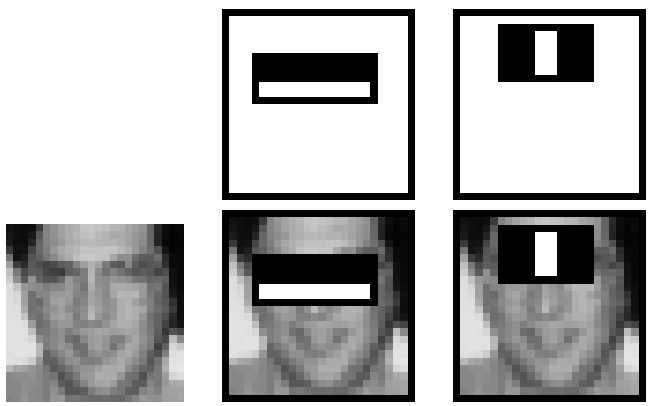
\includegraphics[width=.65\textwidth]{figures/CV_Example.png}
    \caption{Anwendung von AdaBoost bei Computer Vision:
        Das erste Merkmal von AdaBoost misst den Intensitätsunterschied
        zwischen der Augenregion und den oberen Wangen,
        wobei die Augen oft dunkler sind. Das zweite Merkmal vergleicht die
        Intensität der Augen mit der Nasenbrücke.\cite{viola2001rapid}}
\end{figure*}